\documentclass[letterpaper,10pt]{article}

\usepackage{titling}
\usepackage{listings}
\usepackage{url}
\usepackage{setspace}
\usepackage{subfig}
\usepackage{sectsty}
\usepackage{pdfpages}
\usepackage{colortbl}
\usepackage{multirow}
\usepackage{relsize}
\usepackage{amsmath}
\usepackage{fancyvrb}
\usepackage{amsmath,amssymb,amsthm,graphicx,xspace}
\usepackage[titlenotnumbered,noend,noline]{algorithm2e}
\usepackage[compact]{titlesec}
\usepackage{paratype} 
\usepackage[T1]{fontenc}
\usepackage{tikz}
\usetikzlibrary{arrows,automata,shapes,trees,matrix,chains,scopes,positioning,calc}
\tikzstyle{block} = [rectangle, draw, fill=blue!20, 
    text width=2.5em, text centered, rounded corners, minimum height=2em]
\tikzstyle{bw} = [rectangle, draw, fill=blue!20, 
    text width=4em, text centered, rounded corners, minimum height=2em]

\definecolor{namerow}{cmyk}{.40,.40,.40,.40}
\definecolor{namecol}{cmyk}{.40,.40,.40,.40}

\let\LaTeXtitle\title
\renewcommand{\title}[1]{\LaTeXtitle{\textsf{#1}}}


\newcommand{\handout}[5]{
  \noindent
  \begin{center}
  \framebox{
    \vbox{
      \hbox to 5.78in { {\bf ECE254: Operating Systems and Systems Programming } \hfill #2 }
      \vspace{4mm}
      \hbox to 5.78in { {\Large \hfill #4  \hfill} }
      \vspace{2mm}
      \hbox to 5.78in { {\em #3 \hfill} }
    }
  }
  \end{center}
  \vspace*{4mm}
}

\newcommand{\lecture}[3]{\handout{#1}{#2}{#3}{Lecture #1}}
\newcommand{\tuple}[1]{\ensuremath{\left\langle #1 \right\rangle}\xspace}

\addtolength{\oddsidemargin}{-1.000in}
\addtolength{\evensidemargin}{-0.500in}
\addtolength{\textwidth}{2.0in}
\addtolength{\topmargin}{-1.000in}
\addtolength{\textheight}{1.75in}
\addtolength{\parskip}{\baselineskip}
\setlength{\parindent}{0in}
\renewcommand{\baselinestretch}{1.5}
\newcommand{\term}{Spring 2015}

\singlespace


\begin{document}

\lecture{ 5 --- Process State }{\term}{Jeff Zarnett}

\section*{Process State}

The OS is responsible for determining which programs run when and how to allocate resources. The current state of the process is therefore important information. To maintain the state of the process the PCB has a variable, but we will think about this as a finite state machine (FSM): there are a limited number of states and defined transitions between them. 

\subsection*{The Two-State Model}

Let us begin with the simplest possible model: the two state model. At any time, either a process is executing, or it is not. Thus we have the two states: 

\begin{enumerate}
	\item \textbf{Running:} Actively executing right now.
	\item \textbf{Not Running:} Not currently executing.
\end{enumerate}

When a new process is created, the PCB is allocated and the state of the process is Not Running. Whatever process is currently running, and when the process that currently running is finished or a process switch takes place, the running program's state is changed to Not Running, a new process is selected to run (according to scheduling), and it is put in the Running state while it executes.

\begin{center}
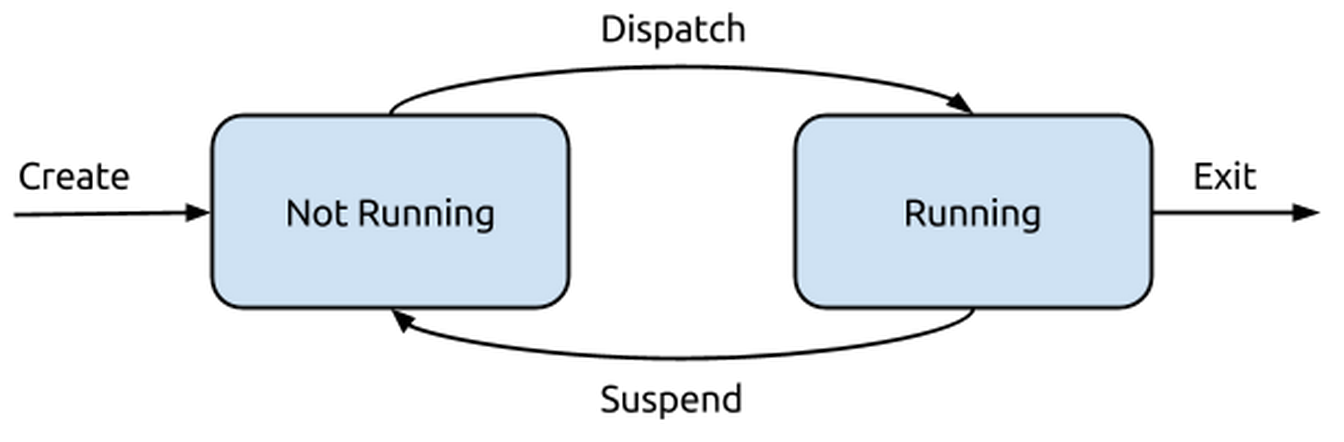
\includegraphics[width=0.65\textwidth]{images/2-state-model.png}\\
State diagram for the two state model.
\end{center}

There are the following transitions in the diagram:
\begin{itemize}
	\item \textbf{Create:} The process is created and enters the Not Running state.
	\item \textbf{Dispatch:} A process that is not currently running begins executing and moves to the Running state.
	\item \textbf{Suspend:} A running program pauses execution, for whatever reason, and moves to the Not Running state.
	\item \textbf{Exit:} A running program finishes, reaching the \texttt{exit}, and can be removed from the list of processes.
\end{itemize}


Thes two-state model, is, however, inadequate. It assumes that every process is constantly ready to run, which is not a safe assumption. We will need a way to indicate that a process is not ready to run, and thus a third state.

\subsection*{The Three-State Model}

A program that requests a resource like I/O or memory may not get it right away. This is not to say the program will never get it, just that it does not have it right now. Sometimes the program needs user input, and as far as the computer is concerned, the user moves at glacial speed. In any case, the program wants to continue but cannot until it gets what it is waiting for.  If the scheduler picks a process that is waiting for user input, nothing will be happening while the program is waiting for input, so the CPU's time would be wasted. Thus, we should be able to mark a process as ``not ready to proceed'', and we then go to a three-state model:

\begin{enumerate}
 \item \textbf{Running:} Actively executing right now.
 \item \textbf{Ready:} Not running, but ready to execute if selected by the scheduler.
 \item \textbf{Blocked:} Not running, and not able to run until some event happens.
\end{enumerate}

This new state, Blocked, indicates that the program is not ready to run for lack of a resource. It may also be called the Waiting state. The scheduler will not choose a Blocked process to run, even if the CPU has nothing else to do. Suppose process $P_{n}$ is waiting for user input. When the user input is received, an interrupt is generated and the interrupt handler runs. The handler takes the input from the I/O device (keyboard), delivers it to $P_{n}$, then moves the state of $P_{n}$ to Ready.

\begin{center}
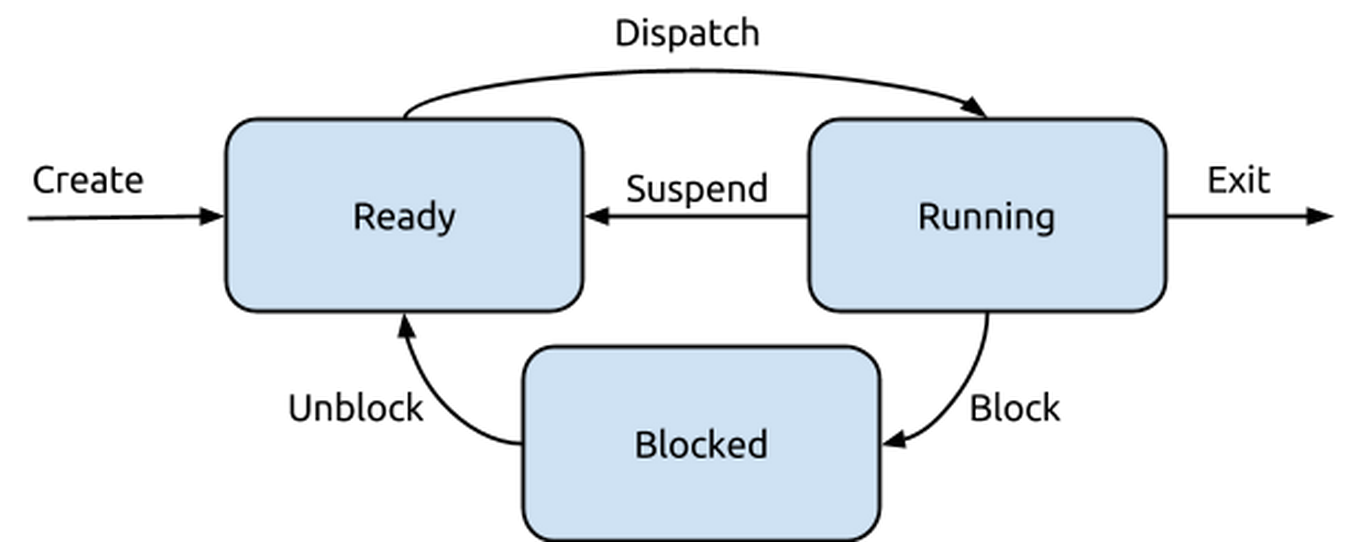
\includegraphics[width=0.65\textwidth]{images/3-state-model.png}\\
State diagram for the three-state model.
\end{center}

There are six transitions in the diagram:
\begin{itemize}
	\item \textbf{Create:} The process is created and enters the Ready state.
	\item \textbf{Dispatch:} A process that is not currently running begins executing and moves to the Running state.
	\item \textbf{Suspend:} A running program pauses execution, but can still run if allowed, and moves to the Ready state.
	\item \textbf{Exit:} A running program finishes, reaching the \texttt{exit}, and can be removed from the list of processes.
	\item \textbf{Block:} A running program requests a resource, does not get it right away, and cannot proceed.
	\item \textbf{Unblock:} A program, currently blocked, receives the resource it was waiting for; it moves to the Ready state.
\end{itemize}


Though this three state model is good, it does not encompass everything we have already discussed, such as a zombie process. We can still improve on it by adding two additional states. 

\subsection*{The Five-State Model}

Earlier we discussed that a UNIX process may be finished but a zombie, because its parent has not (yet) come by to collect its return value. The process is not ready to run (it has finished running) and it is not waiting for a resource, so it does not qualify for Ready or Blocked. Thus, we need a state to represent that it is finished but not yet cleaned up: Terminated.

The fifth and final state will be the ``New'' state: a process that has just been defined. Suppose a user wants to run a new process. The OS will first perform the necessary administrative tasks: define an identifier for the process, instantiate the PCB object, and put the process in the New state. The OS has created the process but has not committed itself to execution thereof. This may be because the system limits the number of concurrent processes for performance reasons. When the process is in the New state is is typically not in memory, but on disk instead~\cite{osi}.

Thus, with the two new states added, the five states of a process in the system are:

\begin{enumerate}
 \item \textbf{Running:} Actively executing right now.
 \item \textbf{Ready:} Not running, but ready to execute if selected by the scheduler.
 \item \textbf{Blocked:} Not running, and not able to run until some event happens.
 \item \textbf{New:} Just created but not yet added to the list of processes ready to run.
 \item \textbf{Terminated:} Finished executing, but not yet cleaned up (reaped).
\end{enumerate}

With five states, we will have significantly more transitions between the states. The diagram below shows the five-state model:

\begin{center}
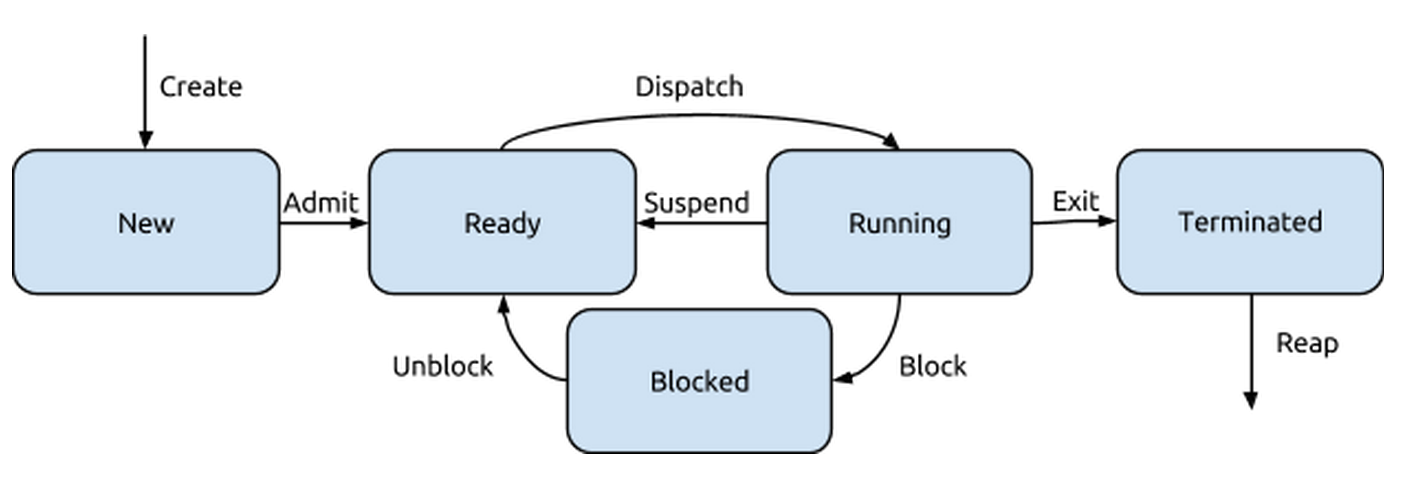
\includegraphics[width=0.85\textwidth]{images/5-state-model.png}\\
State diagram for the five-state model.
\end{center}

There are now eight transitions, most of which are similar to what we have seen before:

\begin{itemize}
	\item \textbf{Create:} The process is created and enters the New state.
	\item \textbf{Admit:} A process in the New state is added to the list of processes ready to start, in the Ready state.
	\item \textbf{Dispatch:} A process that is not currently running begins executing and moves to the Running state.
	\item \textbf{Suspend:} A running program pauses execution, but can still run if allowed, and moves to the Ready state.
	\item \textbf{Exit:} A running program finishes and moves to the Terminated state; its return value is available.
	\item \textbf{Block:} A running program requests a resource, does not get it right away, and cannot proceed.
	\item \textbf{Unblock:} A program, currently blocked, receives the resource it was waiting for; it moves to the Ready state.
	\item \textbf{Reap:} A terminated program's return value is collected by a \texttt{wait} and its resources can be released.
\end{itemize}

There are two additional ``Exit'' transitions that may happen but are not shown. In theory, a process that is in the Ready or Blocked state might transition directly to the Terminated state. This can happen if a process is killed, by the user or by its parent (recall that parent processes can generally kill their children at any time, something the law thankfully does not permit). It may also happen that the system has a policy of killing all the children of a parent process when the parent process dies.




\bibliographystyle{alpha}
\bibliography{254}


\end{document}